% USE PDFLatex!
% to correctly render Swedish characters

\documentclass{popsci}

\usepackage[utf8]{inputenc}
\usepackage[main=swedish, british]{babel}

\usepackage{fancyhdr}
\usepackage{titling}
\usepackage{color}
\usepackage{colortbl}
\usepackage{graphicx}
\usepackage{flushend}
\usepackage{lmodern}
\usepackage{caption}


% Please specify the presentation date
\presentationsdag{2024-01-25}

% use either of these commands to specify the title of your thesis
\examensarbete{Type Checker Generation using Reference Attribute Grammars}
% To create a title in two rows, leave examensarbete blank and fill in examensarbeteTwoRows.
%\examensarbeteTwoRows{Application Specific Instruction-set Processor Using a Parametrizable multi-SIMD}{Synthesizeable Model Supporting Design Space Exploration}
\student{Nicholas Boyd Isacsson}
%\students{Magnus Hultin}{Mr X}
\supervisor{Christoph Reichenback (LTH)}
\examiner{Niklas Fors (LTH)}

% Your pop-sci title should be different (more catchy) than your thesis title
\title{Autogenererad typsäkerhet för programmeringsspråk}


\begin{document}

% not more than 4 rows!
%\theabstract{Applikations-specifika processorer är allt mer vanligt för få ut rätt prestanda med så lite resurser som möjligt. Detta arbete har en parametrisk modell för att kunna testa hur mycket resurser som behövs för en specifik applikation.}
\theabstract{Typkollande är ett vanligt verktyg för att hitta buggar i datorprogram, men är relativt komplicerade att skapa.
Jag har byggt ett program som automatiskt skapar typkollare för program utifrån en kort definition.}


{\noindent
Datorprogram hanterar ofta många olika datatyper, och fel användning av dem är en av de vanligaste buggarna.
För att hitta dessa buggar används typkollare, som systematisk går igenom hela programmet och verifierar varenda användning av variabler eller värden för att se till att rätt datatyp använts på rätt plats.

\begin{figure}[!bth] % Use pictures in your pop-vet!
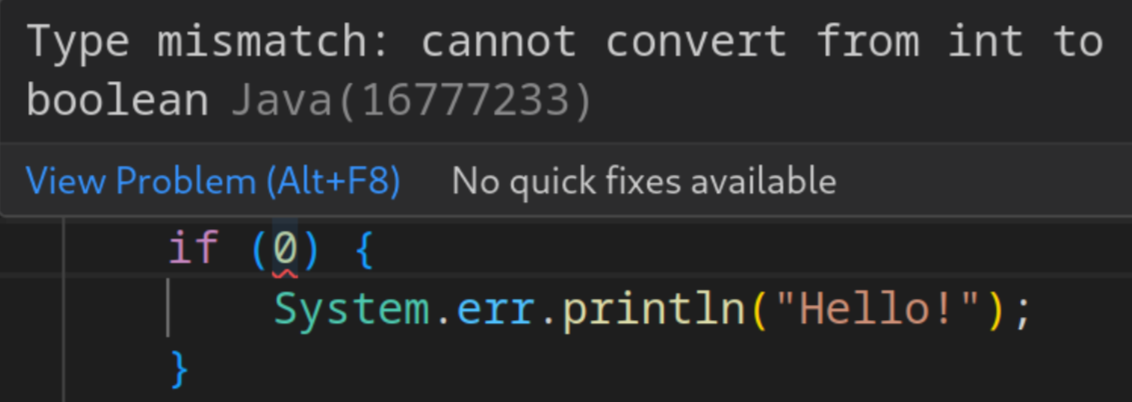
\includegraphics[width=\columnwidth]{typeerror.png}
\caption*{Ett typfel i ett vanligt programmeringsspråk, där en siffra används istället för ett booleskt (sant/falskt) värde.}
\end{figure}

Dessa typkollare är dock komplicerade att skapa, och är ofta starkt kopplade till ett specifikt programmeringsspråk.
Det innebär att varenda programmeringsspråk behöver skapa sin egen typkollare, och leder till en otrolig mängd upprepat arbete.
I mitt arbete har jag skapat ett verktyg för att generera typkollare per automatik, utifrån en kort och koncis definition av programmets regler.

Detta görs genom att baka in kod i ett av mellanleden när programmet omvandlas från människoskriven text till maskinexekverbar kod.
%Detta mellanled representerar programmets beteende, utan att ha med alla detaljer om hur exakt programmet är skrivet.
Mellanledet har en struktur lik ett släktträd där allt härstammar ifrån roten, med grenar som representerar olika kodstrukturer, och som i sig kan delas av i flera grenar.


Därmed kan vi enkelt skapa typkollare för nya språk på ett kortfattat vis, genom att bara definiera vilka regler som ska finnas och inte behöva fundera över hur man implementerar dem.
Det underlättar också om man vill göra förändringar i systemet, eftersom det är mycket lättare att ändra de koncisa reglerna än att ändra de många raderna kod som kan krävas för att implementera den.

I nuläget är programmet ganska begränsat i hur komplicerade typkollare det kan generera, och skulle inte kunna appliceras på något av de stora, kända programmeringsspråken.
Däremot klarar det flera exempel från forskningslitteraturen, och tillvägagångssättet har dock visats vara flexibelt och utbyggbart.
Man borde alltså kunna vidareutveckla programmet för ett bredare stöd i framtiden.


%För att öka prestandan i dagens processorer finns det vektorenheter och flera kärnor i processorer. Vektorenheten finns till för att kunna utföra en operation på en mängd data samtidigt och flera kärnor gör att man kan utföra fler instruktioner samtidigt. Ofta är processorerna designade för att kunna stödja en mängd olika datorprogram. Detta resulterar i att det blir kompromisser som kan påverka prestandan för vissa program och vara överflödigt för andra. I t.ex. videokameror, mobiltelefoner, medicinsk utrustning, digital kameror och annan inbyggd elektronik, kan man istället använda en processor som saknar vissa funktioner men som istället är mer energieffektiv. Man kan jämföra det med att frakta ett paket med en stor lastbil istället för att använda en mindre bil där samma paketet också skulle få plats.
%
%I mitt examensarbete har jag skrivit en modell som kan användas för att snabbt designa en processor enligt vissa parametrar. Dessa parametrar väljs utifrån vilket eller vilka program man tänkta köra på den. Vissa program kan t.ex. lättare använda flera kärnor och vissa program kan använda korta eller längre vektorenheter för dess data.
%
%%För att kunna välja vilken typ av processor som är rätt för den specifika applikationen krävs det ofta att man snabbt kan testa olika prototyper. Att implementera dessa till hårdvara kan ofta vara tidskrävande och ifall det visar sig att implementationen inte klarar dem kraven man ställt för prestanda och energieffektivitet, måste man designa för nya parametrar och mer tid har blivit slösat. %Om den här processen istället kan göras automatiskt utifrån dessa design-parametrar kan man teoretiskt spara en massa tid.
%Modellen testades med olika multimedia program. Den mest beräkningsintensiva och mest upprepande delen av programmen användes. Dessa kallas för kärnor av programmen. Kärnorna som användes var ifrån MPEG och JPEG, som används för bildkomprimering och videokomprimering.
%
%\begin{figure}[!bth] % Use pictures in your pop-vet!
%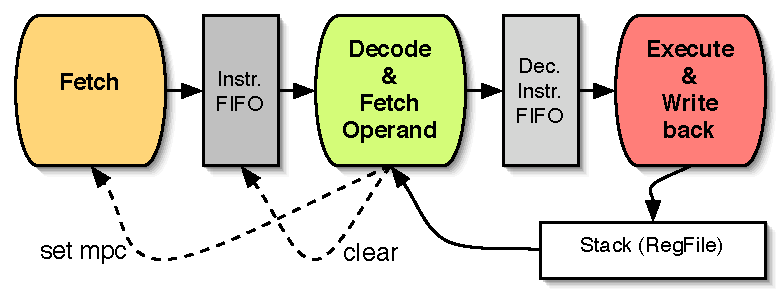
\includegraphics[width=\columnwidth]{samplePic.pdf} 
%%\caption{En fin bild}
%\end{figure}
%Resultatet visar att det finns en prestanda vinst jämfört med generella processorer men att detta också ökar resurserna som behövs. Detta trots att den generella processorn har nästan dubbelt så hög klockfrekvens än dem applikations-specifika processorerna. Resultatet visar också att schemaläggning av instruktionerna i programmen spelar en stor roll för att kunna utnyttja resurserna som finns tillgängliga och därmed öka prestandan. Med den schemaläggningen som utnyttjade resurserna bäst var prestandan minst 79\% bättre än den generella processorn.
}

\end{document}
